

% \begin{figure}[p]
    
%     \begin{minipage}{\textwidth}
%         \begin{mdframed}
%             \label{alg:one-query-ppwps}
%             \begin{center}
%                 {\bf Query Protocol for a Single Query $x$: $\SingleQuery(x,
%                 \sk, p_{\sk}, r, p_r)$.
%                     %\andy{Is it not $O(\sqrt{n})$?}
%                 }
%             \end{center}
            
%             \parhead{Client's input:}
%             %Suppose the client has the following inputs:
%             \begin{itemize}
%                 \item A secret key $\sk$ of a $\PPWPS$ assuming $x\in \Set(\sk)$
%                 \item The parity of $\Set(\sk)$ is assumed to be $p_{\sk}$;
%                 \item A random index $r$ in $x$'s chunk such that the  $\DB[r]$
%                 is assumed to be $p_r$.
%             \end{itemize}
            
%             %\parhead{Suppose the client has a hint $$} When a query $x \in \{0,
%             %1, \ldots, n-1\}$ arrives, \Client performs the following: 
%             \begin{enumerate}[leftmargin=5mm,itemsep=1pt]
%                 \item 
%                 {\bf Step 1: (Client)}

%                 \begin{enumerate}[leftmargin=5mm,itemsep=1pt]

%                         \item Run $(\sk',j)\gets\Program(\sk,\chunk(x),r\text{ mod } \sqrt{n})$
%                         \item Send $\sk'$ to server
                    
%                 \end{enumerate}
                
%                 \newpage
                
%                 \item 
%                 {\bf Step 2: (Server)}
                
%                 Upon receiving $\sk'$, compute $(S_1,S_2,\ldots,S_L)\gets \ListDecode(\sk')$. For each $b\in [L]$, compute the parity of the elements of $\DB$ indexed by $S_b$, i.e., $\beta_b=\oplus_{i\in S_b}\DB[i]$. Send $(\beta_1,\ldots,\beta_L)$ to client.

%                 % \begin{enumerate}
%                 %     \item For $b\in \{0,\dots,n^{1/4}-1\}$:
%                 %     \begin{enumerate}
%                 %         \item Expand $k'_b$ to $n^{1/4}$ offsets and consider
%                 %         them being the corresponding index offsets in chunk $\{b
%                 %         \cdot n^{1/4}, \ldots, (b + 1)\cdot n^{1/4} -1\}$.
%                 %         Compute the xor-sum of the database values for those
%                 %         indices as 
%                 %         \[
%                 %         \alpha_b=\xor_{c\in \{0,\dots,n^{1/4}-1\}} \DB[(c + bn^{1/4})\sqrt{n} + \PRF_2(k'_b, c)].
%                 %         \]
%                 %         \item Consider $(\delta'_0,\dots,\delta'_{j,n^{1/4}-1})$
%                 %         as the corresponding index offsets in chunk $\{b \cdot
%                 %         n^{1/4}, \ldots, (b + 1)\cdot n^{1/4} -1\}$. Compute the
%                 %         xor-sum of the database values for those indices as 
%                 %         \[
%                 %         \beta_b=\xor_{c\in \{0,\dots,n^{1/4}-1\}} \DB[(c + bn^{1/4})\sqrt{n} + \delta_c].
%                 %         \]
%                 %     \end{enumerate}
                    
%                 %     \item Return $(\alpha_0,\dots,\alpha_{n^{1/4}-1}),
%                 %     (\beta_0,\dots,\beta_{n^{1/4}-1})$ to the client.
%                 % \end{enumerate}
                
                
%                 \item 
%                {\bf Step 3: (Client)}

%                Upon receiving $(\beta_1,\ldots,\beta_L)$, output $p_\sk\xor  p_r\xor\beta_{j}$.
%             \end{enumerate}
%         \end{mdframed}
%     \end{minipage}
%     \caption{Query Protocol for a single query that reduces communication to
%     $O(n^{1/4})$. This is used as a sub-routine in the sublinear single server
%     PIR scheme presented in Section~\labelcref{sec:nquarter}.}
%     \label{fig:single-query-ppwps}
% \end{figure}

% \begin{figure}[p]
%     \begin{minipage}{\textwidth}
%         \begin{mdframed}
%             \label{alg:one-query-ppwps-two}
%             \begin{center}
%                 {\bf Two-Server Scheme}
%             \end{center}

%             \parhead{Offline preprocessing.} 
%             %\ \\[-6pt]
%             \begin{itemize}[leftmargin=3mm,itemsep=1pt]
%                 \item 
%                 \Client samples $M_1=2\sqrt{n}\log \kappa \cdot \alpha(\kappa)$
%                 $\PPWPS$ keys denoted $\psk_1, \dots, \psk_{M_1} \in \{0,
%                 1\}^\lambda$ for the hint table.
%                 %, where $M_1=\sqrt{n}\log \kappa \cdot \alpha(\kappa)$. , such
%                 %that $\alpha(n)=\omega(1)$. \elaine{TODO: fix params}
%                 % Initialize the parities $p_1,\dots,p_{M_1}$ to zeros.
                
%                 %\elaine{TODO: notation inconsistent with earlier text}
                
%                 \item For each $i\in [M_1]$, send $\Set(\sk_i)$ to the right server and receive their parities $p_1,\ldots,p_{M_1}$. Let $T := \{(\psk_i, p_i )\}_{i \in
%                 [M_1]}$ denote the client's {\it hint table}.
%                 \item For each chunk $j\in \{0,\ldots,\sqrt{n}-1\}$, sample 
%                 $M_2=3\log \kappa \cdot \alpha(\kappa)$ different $r_1$'s in each chunk, and query them to the left server. Store the tuples $(r_1,\DB[r_1])$. Similarly, sample 
%                 $M_2=3\log \kappa \cdot \alpha(\kappa)$ different $r_2$'s in each chunk, and query them to the right server. Store the tuples $(r_2,\DB[r_2])$.
%                 These are the replacement entries.
%             \end{itemize}
            
%             \parhead{Online query for index $x \in \{0, 1, \ldots, n-1\}$.}
            
%             \begin{enumerate}[leftmargin=5mm,itemsep=1pt]
%                 \item 
%                 {\bf Step 1: (Client)}

%                 \begin{enumerate}[leftmargin=5mm,itemsep=1pt]
%                         \item Find a hint $(\sk,p)$ in the hint table such that $x\in \Set(\sk)$. Find $r_1$ among the replacement entries stored from the left server and $r_2$ among replacement entries stored by the right server such that $r_1,r_2$ are in the chunk of $x$.
%                         \item Run $(\sk_1',j_1)\gets\Program(\sk,\chunk(x),r_2\text{ mod } \sqrt{n})$
%                         \item Sample $\sk_2$ such that $x\in\Set(\sk_2)$.
%                         \item Run $(\sk_2',j_2)\gets\Program(\sk_2,\chunk(x),r_1\text{ mod } \sqrt{n})$
%                         \item Send $\sk_1'$ to left server, $\sk_2'$ to right server
                    
%                 \end{enumerate}
                
%                 \newpage
                
%                 \item 
%                 {\bf Step 2: (Left and Right Server)}
                
%                 Upon receiving $\sk'$, compute $(S_1,S_2,\ldots,S_L)\gets \ListDecode(\sk')$. For each $b\in [L]$, compute the parity of the elements of $\DB$ indexed by $S_b$, i.e., $\beta_b=\oplus_{i\in S_b}\DB[i]$. Send $(\beta_1,\ldots,\beta_L)$ to client.

%                 \item
%                {\bf Step 3: (Client)}

%                Upon receiving $(\beta_{1,1},\ldots,\beta_{L,1})$ from left server and $(\beta_{1,2},\ldots,\beta_{L,2})$ from right server, compute $y=p_\sk\xor  \DB[r_2]\xor\beta_{j_1,1}$ and compute $p_2=\DB[r_1]\xor \beta_{j_2,2}\xor y$. Return $y$, replace $(\sk,p)$ with $(\sk_2,p_2)$ in the hint table.
%             \end{enumerate}
%         \end{mdframed}
%     \end{minipage}
%     \caption{Two-server preprocessing PIR with $\widetilde{O}_\lambda(n^{1/4})$ online communication, $\widetilde{O}_\lambda(n^{1/2})$ online server computation without public-key cryptography}
%     \label{fig:two-server-ppwps}
% \end{figure}
\section{Alternate overview?}

\subsection{Starting point: $\Piano$~\cite{piano}} 
We start by recalling the
high level ideas involved in a the $\Piano$ construction that supports a single
query with $O(\sqrt{n})$ online communication.

Let the database be $\DB$  of size $n$, indexed by $0,\ldots,n-1$. Divide the
database into $\sqrt{n}$ chunks, where chunk $i$ contains the indices of
$\{i\sqrt{n},i\sqrt{n}+1,\dots,(i+1)\sqrt{n}-1\}$. We define
$\chunk(x)=\left\lfloor \frac{x}{\sqrt{n}}\right\rfloor$. During the
preprocessing phase, the client generates many random sets $S_1,\dots,S_{M_1}$.
Each random set will contain exactly one random index from each chunk and have
$\sqrt{n}$ indices. The client stores the parities for those sets. For example,
$p_1=\xor_{x\in S_1}\DB[x]$. Moreover, the client stores, for each chunk,
polylogarithmically many pairs of random indices and their corresponding
database values. These index-value pairs are called replacement pairs.
% For now, we just assume the client can run the preprocessing phase in a server-oblivious fashion. 

In order to make an online query on the index $x$, the client first finds a set
$S$ that $x\in S$. The client only needs to know the parity of $S/\{x\}$
because $\DB[x]=p \xor\left(\xor_{x'\in S/\{x\}}\DB[x']\right)$, and $p$
is known. To achieve this, the client lists out all $\sqrt{n}$ indices in $S$,
replaces $x$ with an unconsumed replacement index, say $y$, from the same chunk
of $x$ and sends these $\sqrt{n}$ indices to the server. The server computes the
parities of these indices and returns a bit $\beta$ to the client, which only
takes $O(\sqrt{n})$ time. Now the client knows $\beta=\left(\xor_{x'\in
S/\{x\}}\DB[x']\right)\xor \DB[y]$. Notice that $\DB[y]$ is known to the
client by preprocessing, so the client can compute the parity of $S/\{x\}$,
and therefore $\DB[x]$.

It is not difficult to prove that if the preprocessing is oblivious to the online server, the
server simply sees a random set that contains $x$ and then $x$ is replaced with
a random index within the same chunk. This set is identically distributed as a
uniformly random set. %Moreover, the during the preprocessing, the client reads
%the database in a streaming fashion, reading a chunk at a time to compute all
%the parities it needs to store. Hence, the preprocessing is indeed oblivious to
%the server. 
Therefore, the scheme is private.

To compress the local storage, the client can use a pseudorandom function
$\PRF:\{0,1\}^\lambda \times \{0,\dots,\sqrt{n}-1\} \to \{0,\dots,\sqrt{n}-1\}$
and represent a set with a $\lambda$-bit key $\sk$. Define $\Set(\sk)$ as
follows: for $j\in \{0,1,\ldots,\sqrt{n}-1\}$, the $j$-th element of
$\Set(\sk)$, denoted as $\Set(\sk)[j]=\PRF(\sk, j) + j\sqrt{n}$. In other words,
we use the PRF to expand the keys to $\sqrt{n}$ \emph{offsets} and the $j$-th
offset is the offset of the random index inside the $j$-th chunk. The client
only needs $\widetilde{O}(\sqrt{n})$ sets, so the client storage cost is
$\widetilde{O}_\lambda(\sqrt{n})$. 



\heading{Privately Programmable Pseudorandom Set with List Decoding.} In this work, we will present a new abstraction of the aforementioned $\Piano$ protocol. To this end, we define a new primitive called \emph{privately programmable pseudorandom set with list decoding}~($\PPWPS$). Our starting point is the notion of pseudorandom sets which provide an algorithm to generate a pseudorandom subset that $S \subset \{0, 1, \ldots, n-1\}$ of size $\sqrt{n}$ 
sampled from the following distribution
$\mcal{D}_n$: the $i$-th element in each set is an uniformly random element in $\{i\cdot \sqrt{n},i\cdot \sqrt{n}+1,\ldots,(i+1)\cdot \sqrt{n}-1\}$.
A privately programmable pseudorandom set with list decoding is a pseudorandom sets with the following additional property:
the set must be \emph{privately programmable and list decodable}, meaning there exist a pair of algorithms $\Program,\ListDecode$ such that 
\begin{itemize}
    \item Given $\sk,\ell,y$, $\Program$ returns a secret key $\sk'$ and an index $j\in \{1,\ldots,L\}$
    \item Given $\sk'$ output by $\Program$, $\ListDecode$ returns a list of $L$ sets such that the $j$-th element in the list of sets is the set $\Set(\sk)$, except with the $\ell$-th element replaced with $y$.
\end{itemize}

\heading{An alternative view of $\Piano$.} 
We present an alternative view of the aforementioned $\Piano$~\cite{piano} protocol through the lens of $\PPWPS$.
The basis of the view is that $S_1,\ldots,S_{M_1}$ generated by the client can be viewed as $\PPWPS$s -- the $\PRF$ keys are the keys for $\PPWPS$. When the client wants to make an online query on index $x$, the client essentially finds a secret key $\sk$ such that $x\in \Set(\sk)$. It programs the secret key $\sk$ at $\chunk(x)$, with a random value $y$ that is in the chunk of $x$, such that it has stored $\DB[y]$ during preprocessing. The result of this programming consists of {\bf 1)} the secret key $\sk'$ which is the set $S'$ 
with $x$ replaced by $y$ {\bf 2)} the index $j$ which equals $\superblock(x)$.  The client sends $\sk'$ to the server, who runs list decoding on this key to obtain the $L=n^{1/2}$ different sets, and sends over their corresponding xor-sums. The client computes the correct answer by xor-ing the $j$-th entry of the list with the parity corresponding to $\sk$ and $\DB[y]$, both of which are known from preprocessing.

Security follows from the pseudorandomness and privacy of programming of the $\PPWPS$. Privacy ensures that the server's view is indistinguishable from a random element sampled from $\mcal{D}_n$ and privacy of programming ensures that the server learns nothing about the location of $x$.

\subsection{Reducing online communication to $\widetilde{O}_\lambda(n^{1/4})$
bits}
 We re-cast the single query scheme for $\Piano$ into this new abstraction of $\PPWPS$ is because it clearly suggests a pathway towards reducing online communication -- construct a $\PPWPS$ scheme where the $\Program$ function generates secret keys that are smaller than $O(n^{1/2})$ bits. Our first main contribution in this work is construction of a $\PPWPS$ scheme where the output the programmed secret key is $O(n^{1/4})$ bits long. That already reduced the communication to $O(n^{1/4})$.

\heading{$\PPWPS$ construction with succinct programmed keys.} In the $\PPWPS$ used in $\Piano$, the programmed key is simply the set representation of the programmed set. For the same pseudorandom set as in $\Piano$, we give a new definition of the $\Program$ procedure that produces more succinct programmed keys. Towards this, we will introduce the notion of {\bf
superblocks}. We group $n^{1/4}$ consecutive chunks into one superblock, so each
superblock contains $n^{3/4}$ indices and there are $n^{1/4}$ superblocks in
total. We define $\superblock(x)=\left\lfloor \frac{x}{n^{3/4}}\right\rfloor$.
Further, we say that the relative location of $\chunk(x)$ in superblock $j$ is
$\chunk(x)-j\cdot n^{1/4}$. 

Our new representation of keys for the $\PPWPS$ will be based on a two-layer construction. At a
high-level, given a key $\sk$, we will first expand that key to $n^{1/4}$
\emph{sub-keys} using one PRF. Each sub-key corresponds to one super-block. It
then uses another PRF to expand each sub-key to $n^{1/4}$ offsets. The offsets
expanded by a particular sub-key are the offsets of the chunks inside its
corresponding superblock. 

Formally, we assume that the $\PRF:\bits^{\lambda}\times \bits^{\frac{\log
n}{2}}\to \bits^{\frac{\log n}{2}}$ is constructed from two different $\PRF$'s
$\PRF_1: \bits^{\lambda}\times \bits^{\frac{\log n}{4}}\to
\bits^{\lambda},\PRF_2:\bits^{\lambda}\times \bits^{\frac{\log n}{4}}\to
\bits^{\frac{\log n}{2}}$ as follows:
\begin{align*}
    \PRF(\sk,x)=\PRF_2(\PRF_1(\sk,\lfloor x / n^{1/4} \rfloor ),x\bmod n^{1/4}).
\end{align*}

% \begin{figure*}
%     \centering
%     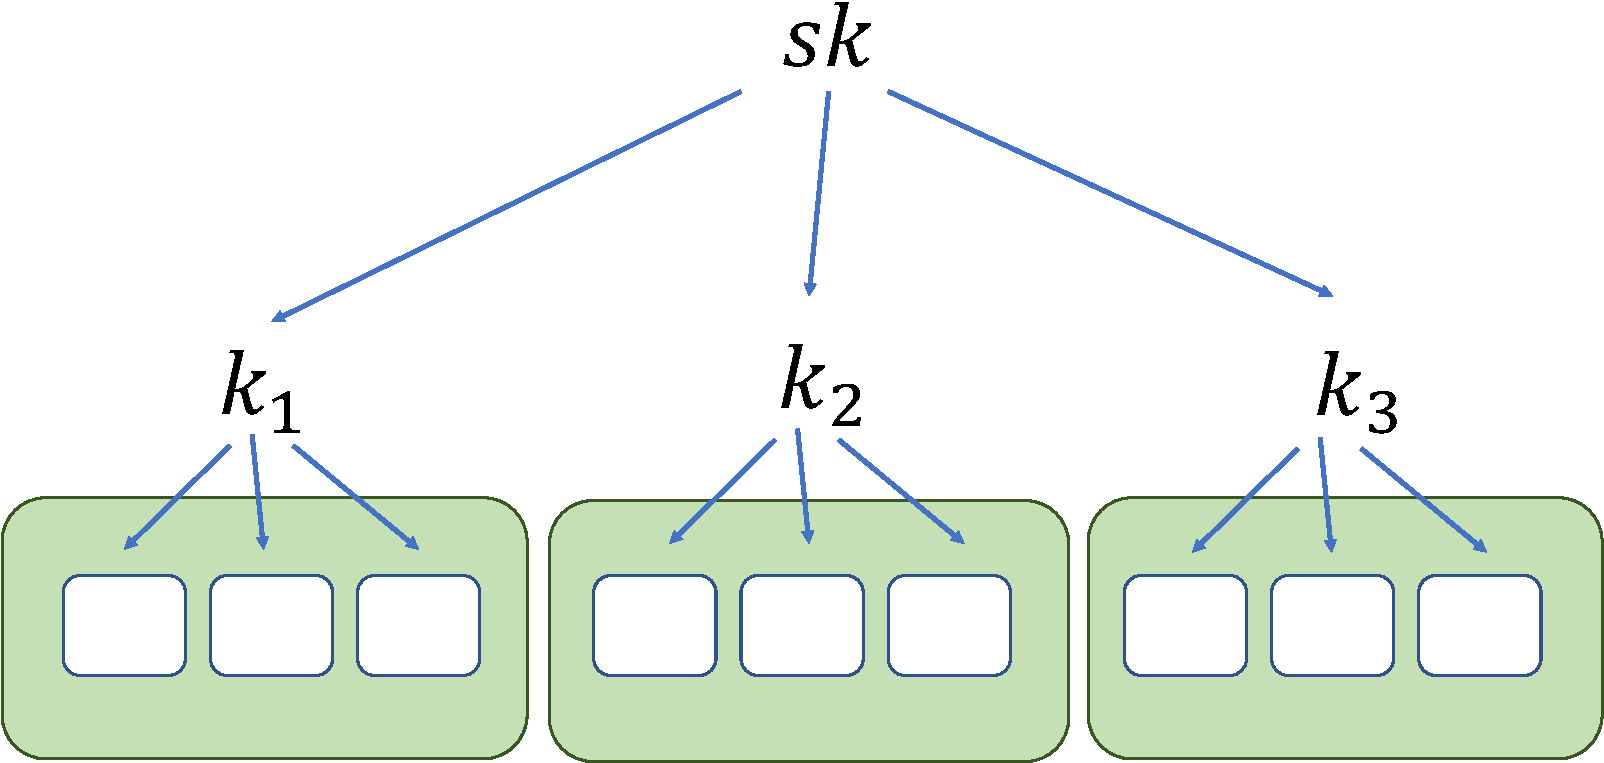
\includegraphics[width=0.6\linewidth]{figs/set-rep.pdf}
%     \caption{Two-layer set representation\label{fig:set-rep}. The first layer key expands to $n^{1/4}$ sub-keys. Each sub-key controls a superblock and expands to $n^{1/4}$ offsets. Each offset in a chunk represents an index.}
% \end{figure*}

%Here, $x[i:j]$ means the bit string from the $i$-th bit to the $(j-1)$-th bit of $x$'s binary representation.

Now, the new $\Program$ procedure will work as follows: it will expand the key $\sk$ into its $n^{1/4}$ sub-keys $k_0,\dots,k_{n^{1/4}-1}$. It will expand the $\superblock(x)$-th
sub-key into $n^{1/4}$ offsets $\delta_0,\dots,\delta_{n^{1/4}-1}$. Let $y$ be a random element in $x$'s chunk and $k'$ be a uniformly random sub-key $k'\getr\{0,1\}^\lambda$. $\Program$ outputs the programmed key to be all the sub-keys $k_0,\dots,k_{n^{1/4}-1}$, except replacing $\superblock(x)$-th key with $k'$ and all the offsets 
replaces $x$'s offset to $y$'s offset and sends those $n^{1/4}$ offsets $\delta_0,\dots,\delta_{n^{1/4}-1}$, except replacing the offset corresponding to $x$ with $y$'s offset. Additionally, $\Program$ returns $\superblock(x)$ as the index $j$.

With this new definition of $\Program$, we also need to modify the definition of $\ListDecode$. On input the sub-keys $k_0',k_1',\ldots,k_{n^{1/4}-1}'$, and offsets $\delta_0',\delta_1',\ldots,\delta_{n^{1/4}-1}'$, 
$\ListDecode$ expands all the sub-keys to get $n^{1/4}$ offsets for each of them. For $i\in \{0,1,\ldots,n^{1/4}-1\}$, the server computes $S_i$ by considering the offsets for all superblocks other than the $i$-th superblock to be the offsets for their corresponding sub-keys and the offsets $\delta_0',\delta_1',\ldots,\delta_{n^{1/4}-1}'$ as the offsets of the $i$-th superblock.


We can now simply plug this new $\PPWPS$ construction into the existing structure of the single query protocol of $\Piano$ and get a protocol with $O(n^{1/4})$ online communication. In Section~\labelcref{sec:ppps} we formally define $\PPPS$ and describe and prove the security of our construction. 

\subsection{Supporting multiple queries in the online phase} 

Thus far, we have
given a new, low-communication protocol that handles only one query. We now want
to make $Q=\sqrt{n}/2$ queries with just one offline phase. For convenience, we
first make some assumptions about the queries without loss of generality, which
are also made in $\Piano$:
\begin{itemize}
    \item \textit{The client does not make repeated queries.} This can be ensured 
    by requiring the client to store a local cache of size $Q$ for caching the
    most recent $Q$ queries. If the client wants a repeated query, it can lookup
    in the cache and make a dummy query.
    
    \item \textit{The queries the client makes are on random indices.} This is a relatively
    strong assumption. However, we argue that it can be made without loss of
    generality and can be done by letting the client and the server agree on a
    pseudorandom permutation (PRP)~\cite{prp1,prp2} upfront and the server can
    permute the database according to the PRP. Another option is let the server
    build the database as a key-value storage and use a cuckoo hash
    table~\cite{cuckoo1,cuckoo2} directly based on a PRF to locate the queries.
    Notice that, in both implementations, the client can still make queries
    adaptively depending on the real query sequnce and the responses, which is
    sufficient for practical usage. Then, as long as the client makes the
    queries independent of the randomness of the PRP/PRF, those queries can be
    considered as uniformly random. This assumption is only needed for the
    correctness.
\end{itemize}

% What was d

% In order to support multiple queries, the key idea that had been used in
% $\Piano$ was to ``refresh" the consumed hint by re-programming a fresh hint in a
% way that does not change the distribution of the hints. Here, while our high
% level goal will be the same, our strategy to do it would be significantly
% different. The reason why the approach used in $\Piano$ does not translate here
% is because of the following tension. Since in this new protocol we compress
% bandwidth by making the client send only \emph{sub-keys} for the superblocks,
% re-programming the hint while still having this compression would make
% distribution of the client's future messages depend on the current query, which
% violates privacy. Therefore, we seem to require newer ideas to avoid this issue.

We will first show how to handle multiple queries when we have two-servers. We will use the additional server \emph{only} for ``refreshing'' the $\PPWPS$ after they have been consumed during an online query. The key idea is suppose $x$ was the queried index and the query returned answer $p_x$, we will sample a new secret $\PPWPS$ key $\sk'$ subject to $x\in\Set(\sk')$. We will program this key using $\Program$ at $\chunk(x)$.